%%%%%%%%%%% NO OLVIDAR COLOCAR ESTE COMENTARIO CON EL NUMERO DE EJERCICIO %%%%%%%%%%%%%
%%%%%%%%%%%%%%%%%%% EJERCICIO 3 %%%%%%
\textbf{Ejemplo 3. Selección entre dos proyectos de puente}\newline
Se presentan dos proyectos de puente. La alternativa A es un puente colgante con costo inicial de COP 850.000.000; el mantenimiento de la plataforma de asfalto cuesta COP 3.000.000 el primer año y aumenta COP 2.000.000 cada año. Cada cinco años se cambian los cables a un costo de COP 100.000.000. La alternativa B es un puente de concreto con costo inicial de COP 900.000.000; cada tres años se reacondicionan las bases por COP 25.000.000 y el mantenimiento anual es fijo de COP 5.000.000. Use una tasa del 24\% periódica anual vencida (pav).\\

\textbf{Solución.}\\

\begin{center}
	\renewcommand{\arraystretch}{1.5}% Margenes de las celdas
	\small% Tamaño de letra de la tabla para que quepan las expresiones con COP
	\begin{longtable}[H]{|c|c|c|}
		\hline
		\rowcolor[HTML]{FFB183}
		%%%%% INICIO ASIGNACIÓN FECHA FOCAL %%%%%%%
		\multicolumn{3}{|c|}{\cellcolor[HTML]{FFB183}\textbf{1. Asignación período focal}} \\ \hline
		\multicolumn{3}{|c|}{$pf = 0\text{ pav}$} \\ \hline
		
		%%%%% INICIO DECLARACIÓN DE VARIABLES %%%%%%%
		\rowcolor[HTML]{FFB183}
		\multicolumn{3}{|c|}{\cellcolor[HTML]{FFB183}\textbf{2. Declaración de variables}} \\ \hline
		\multicolumn{1}{|c|}{\cellcolor[HTML]{FFB183}\textbf{Valores monetarios}} &
		\multicolumn{1}{c|}{\cellcolor[HTML]{FFB183}\textbf{Valores no monetarios}} &
		\multicolumn{1}{c|}{\cellcolor[HTML]{FFB183}\textbf{Incógnitas}} \\ \hline
		
		$P_A = \text{COP } 850.000.000$ & $i = 24\%\text{ pav}$ & $CAUE_A = \text{? COP/año}$ \\
		$R_{1,A} = \text{COP } 3.000.000$ & $n_A = 5\text{ pav}$ & $CAUE_B = \text{? COP/año}$ \\
		$L_A = \text{COP } 2.000.000$ & $n_B = 3\text{ pav}$ & \\
		$C_{\text{cables},A} = \text{COP } 100.000.000\text{ en } t = 5$ & & \\
		$P_B = \text{COP } 900.000.000$ & & \\
		$R_B = \text{COP } 5.000.000/\text{año}$ & & \\
		$C_{\text{reac},B} = \text{COP } 25.000.000\text{ en } t = 3$ & & \\ \hline

		%%%%% INICIO FLUJO DE CAJA
		\rowcolor[HTML]{FFB183}
		\multicolumn{3}{|c|}{\cellcolor[HTML]{FFB183}\textbf{3. Diagrama de flujo de caja}} \\ \hline
		
		\multicolumn{3}{|c|}{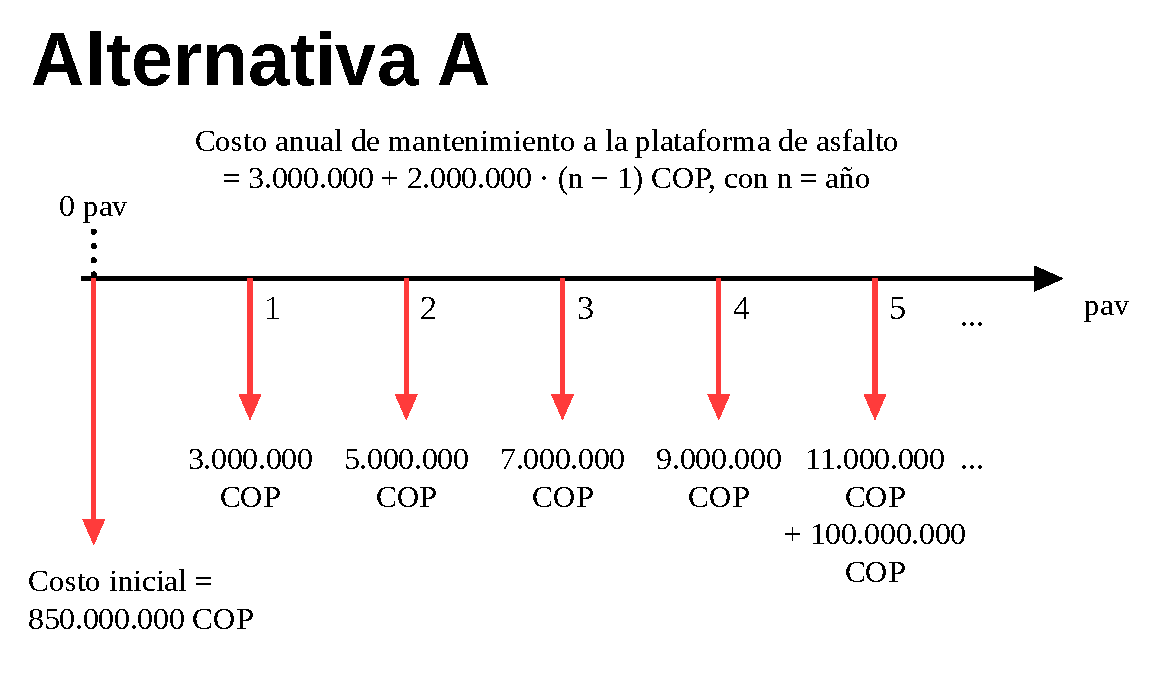
\includegraphics[trim=-5 -5 -5 -5, width=12cm, keepaspectratio]{10_Capitulo/img/ejemplos/PDFs/3/Ejemplo_3_A.pdf}}\\ \hline
		\multicolumn{3}{|c|}{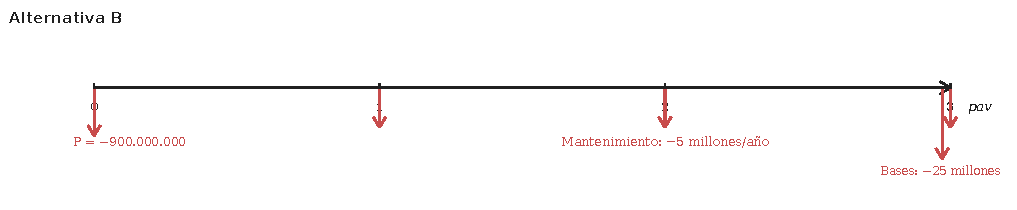
\includegraphics[trim=-5 -5 -5 -5, width=12cm, keepaspectratio]{10_Capitulo/img/ejemplos/PDFs/3/Ejemplo_3_B.pdf}}\\ \hline
		\multicolumn{3}{|p{14cm}|}{\small En A, el flujo de mantenimiento es un gradiente aritmético: $R_{t,A} = 3.000.000 + (t-1)(2.000.000)$, para $t = 1, 2, 3, 4, 5$. En B, el mantenimiento es uniforme y el reacondicionamiento ocurre al final del año 3.} \\ \hline

		%%%%% INICIO DECLARACIÓN FORMULAS
		\rowcolor[HTML]{FFB183}
		\multicolumn{3}{|c|}{\cellcolor[HTML]{FFB183}\textbf{4. Declaración de fórmulas}} \\ \hline

		\multicolumn{3}{|c|}{$CAUE = VPN \times (A/P, i, n)$}\\ 
		\multicolumn{3}{|c|}{$VPN = \sum F_t(1+i)^{-t} \quad \text{(cada egreso se registra con signo negativo)}$}\\
		\multicolumn{3}{|c|}{$A/P = \dfrac{i(1+i)^n}{(1+i)^n - 1} \quad ; \quad A/F = \dfrac{i}{(1+i)^n - 1}$}\\
		\hline

		%%%%%% INICIO DESARROLLO MATEMÁTICO
		\rowcolor[HTML]{FFB183}
		\multicolumn{3}{|c|}{\cellcolor[HTML]{FFB183}\textbf{5. Desarrollo matemático}} \\ \hline

		\multicolumn{3}{|l|}{\textbf{Alternativa A: puente colgante}} \\
		\multicolumn{3}{|p{14cm}|}{Primero se calcula el valor presente del gradiente de mantenimiento:} \\
		\multicolumn{3}{|p{14cm}|}{$VP_{\text{mant},A} = \dfrac{3.000.000}{1{,}24} + \dfrac{5.000.000}{1{,}24^2} + \dfrac{7.000.000}{1{,}24^3} + \dfrac{9.000.000}{1{,}24^4} + \dfrac{11.000.000}{1{,}24^5} = \text{COP } 16.901.534{,}21$.} \\
		\multicolumn{3}{|p{14cm}|}{$CAUE_A = -850.000.000(A/P, 24\%, 5) - VP_{\text{mant},A}(A/P, 24\%, 5) - 100.000.000(A/F, 24\%, 5)$} \\
		\multicolumn{3}{|p{14cm}|}{$CAUE_A = -309.610.557{,}64 - 6.156.345{,}21 - 12.424.771{,}49 = -\text{COP } 328.191.674{,}35/\text{año}$.} \\ \hline

		\multicolumn{3}{|l|}{\textbf{Alternativa B: puente de concreto}} \\
		\multicolumn{3}{|p{14cm}|}{$CAUE_B = -900.000.000(A/P, 24\%, 3) - 5.000.000 - 25.000.000(A/F, 24\%, 3)$} \\
		\multicolumn{3}{|p{14cm}|}{$CAUE_B = -454.246.505{,}72 - 5.000.000 - 6.617.958{,}49 = -\text{COP } 465.864.464{,}21/\text{año}$.} \\ \hline

		\rowcolor[HTML]{FFB183}
		\multicolumn{3}{|c|}{\textbf{Comparación}} \\ \hline
		\cellcolor[HTML]{FFB183} & \cellcolor[HTML]{FFB183}\textbf{A (COP/año)} & \cellcolor[HTML]{FFB183}\textbf{B (COP/año)} \\ \hline
		CAUE & $-328.191.674{,}35$ & $-465.864.464{,}21$ \\ \hline

		%%%%%% INICIO RESPUESTA
		\rowcolor[HTML]{FFB183}
		\multicolumn{3}{|c|}{\cellcolor[HTML]{FFB183}\textbf{6. Respuesta}} \\ \hline

		\multicolumn{3}{|c|}{\parbox{14cm}{\centering\strut Se selecciona la alternativa A. Su costo anual uniforme equivalente es menor: COP 328.191.674,35/año frente a COP 465.864.464,21/año de la alternativa B. La ventaja anual equivalente de A es COP 137.672.789,86.\strut}} \\ \hline
	\end{longtable}
\end{center}

\begin{center}
	\renewcommand{\arraystretch}{1.3}
	\begin{tabular}{|p{14.5cm}|}
		\hline
		\rowcolor[HTML]{FFB183}
		\textbf{Corrección sustancial del ejemplo 3} \\ \hline
		El cálculo original no anualizaba los costos iniciales de COP 850.000.000 y COP 900.000.000, y sumaba directamente costos anuales de mantenimiento. Además, la variable ``$VS$'' se utilizaba para un costo anual, aunque $VS$ corresponde a valor de salvamento. La solución corregida incluye las inversiones iniciales, descuenta los flujos extraordinarios y compara todos los costos en COP/año. \\ \hline
	\end{tabular}
\end{center}

\begin{center}
	\renewcommand{\arraystretch}{1.3}
	\begin{tabular}{|p{14.5cm}|}
		\hline
		\rowcolor[HTML]{FFB183}
		\textbf{Conclusión del capítulo} \\ \hline
		Antes de aplicar el CAUE, verificar que $i$ y $n$ tengan la misma periodicidad y modalidad; identificar la fecha de cada flujo; usar $A/P$ para anualizar un valor presente y $A/F$ para anualizar un valor futuro; y comparar las alternativas con el mismo convenio de signos. \\ \hline
	\end{tabular}
\end{center}
%%%%%%%%%%%%%%%%%%%%%%%%%%FIN EJERCICIO 3 %%%%%%%%%%%%%%%%%%%%%%%%%%%
